\documentclass[final,t]{beamer}
\mode<presentation>
{

  \usetheme{PH}
}
% additional settings
\setbeamerfont{itemize}{size=\normalsize}
\setbeamerfont{itemize/enumerate body}{size=\normalsize}
\setbeamerfont{itemize/enumerate subbody}{size=\normalsize}

%additional packages
\usepackage{times} 
\usepackage{amsmath,amsthm, amssymb, latexsym}
\usepackage{exscale} \boldmath 
\usepackage{booktabs, array}
\usepackage{rotating} %sideways environment 
\usepackage[english]{babel}
\usepackage[latin1]{inputenc}
\usepackage{xspace}
\usepackage{url}
\usepackage{hyperref}
\usepackage{multicol}
\usepackage{xspace}
\usepackage{natbib}
\usepackage{subfig}
\usepackage[orientation=landscape,size=a0,scale=0.85]{beamerposter}
\usepackage{Sweave}

% To produce both postscript and pdf graphics, remove the eps and pdf
% parameters in the next line. Set default plot size to 5 x 3.5 in.

%\listfiles
%\graphicspath{{figures/}}
% Display a grid to help align images
%\beamertemplategridbackground[1cm]

\title{Meta-Analysis of the Fine Particulate Matters-Associated Occupational Health Risks}
\author[1]{Nan-Hung Hsieh$^1$, Shun-Hui Chung$^2$}
\institute[1]{$^1$Department of Veterinary Integrative Biosciences, Texas A\&M  University, College Station, TX\\
$^2$Institute of Labor, Occupational Safety And Health, Ministry of Labor, New Taipei City, Taiwan}

%%%%%%%%%%%%%%%%%%%%%%%%%%%%

\begin{document}
\Sconcordance{concordance:beamerpostertest.tex:beamerpostertest.Rnw:%
1 45 1 1 18 15 1 1 80 1 9 44 0 1 2 2 1 1 9 23 0 1 2 70 1}


\begin{frame}[fragile]
  \begin{columns}[t]

    %-- Column 1 ---------------------------------------------------
    \begin{column}{0.26\linewidth}
      %-- Block 1-1
      \begin{block}{Motivation}
Fine particulate matter (PM) is the recognized risk factor that can cause respiratory and other diseases. Some environmental regulations have been established to protect public people from health concerns. However, it still needs more criterion to understand the fine PM-induced health effects for each occupational population and to further conduct the health protection strategy. This study aims to provide a quantitative summary the fine PM-associated health risk for workers in workplaces. 
      \end{block}
            \begin{block}{Methods}
\textbf{\textit{Literature search.}} Relevant studies were identified in several stages, beginning with a systematic search using the keywords of fine particulate matter, workplace, and occupational in the abstract, with the results restricted to studies of occupational population. An initial search was conducted in July 2015 and updated automatically through December 2015. \textbf{\textit{Inclusion and exclusion criteria.}} studies were included in the current meta-analysis if they provided quantitative risk estimates of hazard ratio, risk ratio, or odds ratio. \textbf{\textit{Statistical analyses.}}  All study estimates were converted to risk ratio to represent the change under fine PM exposure. Estimates from the studies were combined using both fixed-  and random-effects model, which allowed between-study heterogeneity to contribute to the variance.
      \end{block}
      
%-- Block 1-2
\begin{block}{Review of Workplace Fine PM and Occupational Mortality}
\\
% latex table generated in R 3.2.4 by xtable 1.8-2 package
% Tue Feb 28 16:25:58 2017
\begin{tabular}{lllll}
  \hline
Reference & Cohort & Exposure & Cause & CaseNo. \\ 
  \hline
Sjogren et al. & 234 welder & Hexavalent & Ischaemic heart & 10 \\ 
  1987 &  & chromium & disease (IHD) &  \\ 
  Steenland et al. & 92 control dockworkers & Diesel fume & Lung cancer (LC) & 70 \\ 
  1998 & 604 control long-haul &  &  & 609 \\ 
   & drivers &  &  & 121 \\ 
   & 134 control short-haul drivers &  &  &  \\ 
   & 50  control truck &  &  & 37 \\ 
   & mechanics &  &  &  \\ 
   & 143  control other &  &  & 99 \\ 
   & potentially exposed &  &  &  \\ 
  Randem et al. & 8,610 male asphalt & Bitumen fume & Cerebrovascular & 73/214 \\ 
  2003 & workers & and PAH & disease (CBD)/IHD &  \\ 
  Finkelstein et al. & 1,009 Heavy & Diesel fume & CBD/IHD & 38/259 \\ 
  2004 & equipment operators &  &  &  \\ 
   & 271 boilermakers &  &  & 9/59 \\ 
   & 1,533 electricians &  &  & 61/332 \\ 
   & 201 insulators &  &  & 5/34 \\ 
   & 220 painters &  &  & 5/40 \\ 
   & 3,561 plumbers &  &  & 190/876 \\ 
   & 505 sheet metal &  &  & 22/92 \\ 
  Laden et al. & 54,319  male  in the & Diesel fume & CBD/IHD & 167/1,133 \\ 
  2007 & trucking industry &  &  &  \\ 
  Toren et al. & 248,087 male & Diesel fume & CBD/IHD & 423/1,720 \\ 
  2007 & construction workers &  &  &  \\ 
   &  & Asphalt fume &  & 45/171 \\ 
   &  & Metal fume &  & 205/831 \\ 
  Garshick et al. & 29,324 male workers & Diesel fume & LC & 179 \\ 
  2012 & in trucking industry & in diffewrent &  & 202 \\ 
   &  & levels &  & 248 \\ 
  Silverman et al. & 228 control male miners & Diesel fume & LC & 50 \\ 
  2012 & 157 control male miners &  &  & 49 \\ 
   & 123 control male miners &  &  & 50 \\ 
  Costello et al. & 39,412 autoworkers & Metal fume & IHD & 67 \\ 
  2013 &  & in different &  & 68 \\ 
   &  & levels &  & 68 \\ 
   &  &  &  & 67 \\ 
  Mohner et al. & 5,862 potash miners & Diesel fume & LC & 68 \\ 
  2013 &  &  &  &  \\ 
   \hline
\end{tabular}\end{block}
%-- Block 1-3
\begin{block}{Review of Ambient Fine PM and Occupational Mortality}
% latex table generated in R 3.2.4 by xtable 1.8-2 package
% Tue Feb 28 16:25:58 2017
\begin{tabular}{llll}
  \hline
Reference & Cohort & Cause & CaseNo. \\ 
  \hline
Puett et al. 2009 & 66,250 women from the Nurses' Health study & Coronary heart disease & 1,348 \\ 
  Hart et al. 2011 & 53,814 men in the U.S. trucking industry & All-causes & 4,806 \\ 
   &  & Cardiovascular disease & 1,682 \\ 
   &  & Ischemic heart disease & 1,109 \\ 
  Lipsett et al. 2011 & 73,489 women from the California & Cardiovascular disease & 1,630 \\ 
   & Teachers Study &  &  \\ 
  Puett et al. 2011 & 17,545 male from Health Professionals  & All-cause & 2,813 \\ 
   & Follow-Up Study prospective cohort & Cardiovascular disease & 1,661 \\ 
   &  & IHD & 746 \\ 
  Weichenthal et al. & 83,378 subjects included farmers, their  & All-cause & 3,961 \\ 
  2014 & spouses, and commercial pesticide & Cardiovascular disease & 1,055 \\ 
   & applicators. &  &  \\ 
  Ostro et al. 2015 & 133,479 current and former female teachers & All-cause & 6,285 \\ 
   & and administrators & Cardiovascular disease & 2,400 \\ 
   &  & IHD & 1,085 \\ 
  Hart et al. 2015 & 108,767 members of the Nurses' Health  & All-cause & 8,617 \\ 
   & Study 2000-2006 &  &  \\ 
   \hline
\end{tabular}\end{block}
    \end{column}%1

    %-- Column 2 ---------------------------------------------------
    \begin{column}{0.36\linewidth}
      \begin{block}{Workplace Fine PM-associated occupational mortality}
      We summarized the result of the fine PM-associated mortality of respiratory and other diseases, which include lung cancer, ischemic heart disease, and cerebrovascular disease. The result shows that lung cancer has the highest risk ratio with insignificant heterogeneity. Random-effects estimation also indicated the consistencies between studies.
      \vspace{5mm}
      \\
      {\large A) Ischemic Heart Disease Mortality}\\
      \begin{figure}[htb]
      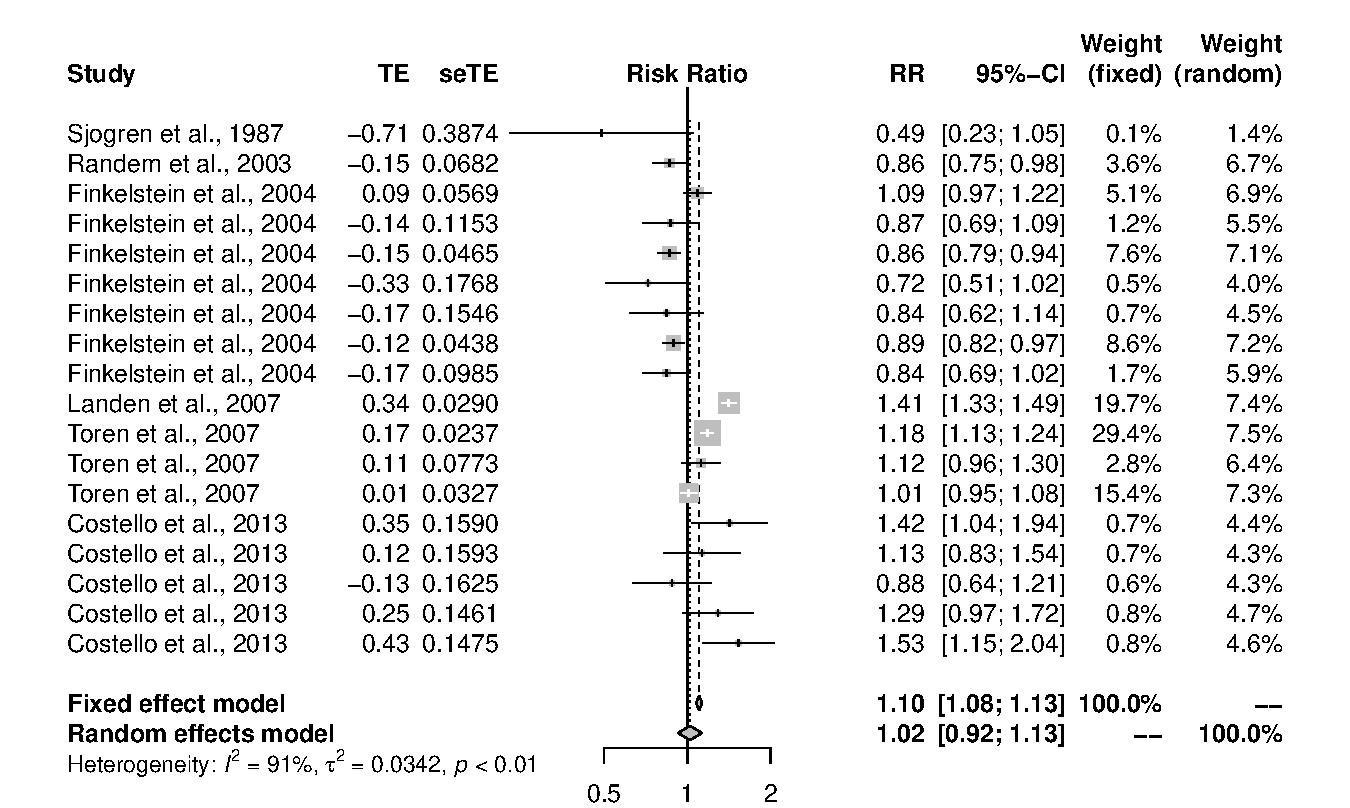
\includegraphics[width=.95\columnwidth]{fig1}
      \end{figure}
      {\large B) Cerebrovascular Disease Mortality}\\
      \begin{figure}[htb]
      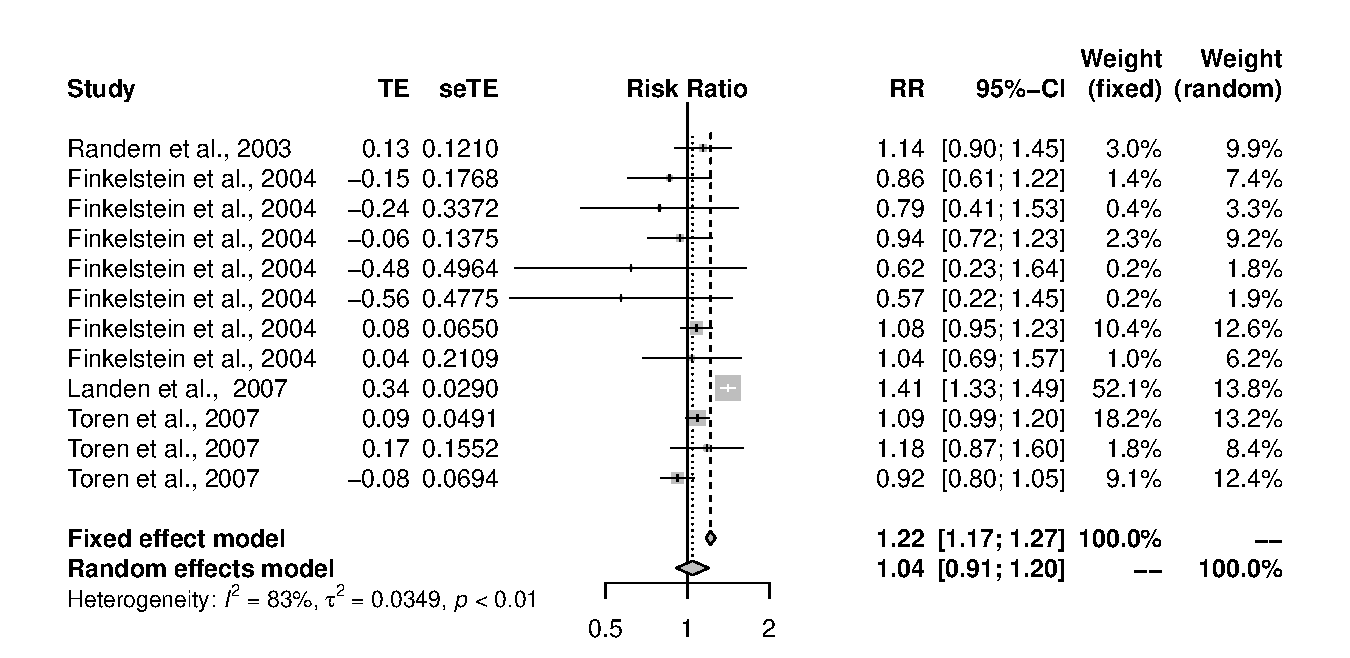
\includegraphics[width=.95\columnwidth]{fig2}
      \end{figure}
      {\large C) Lung Cancer Mortality}\\
      \begin{figure}[htb]
      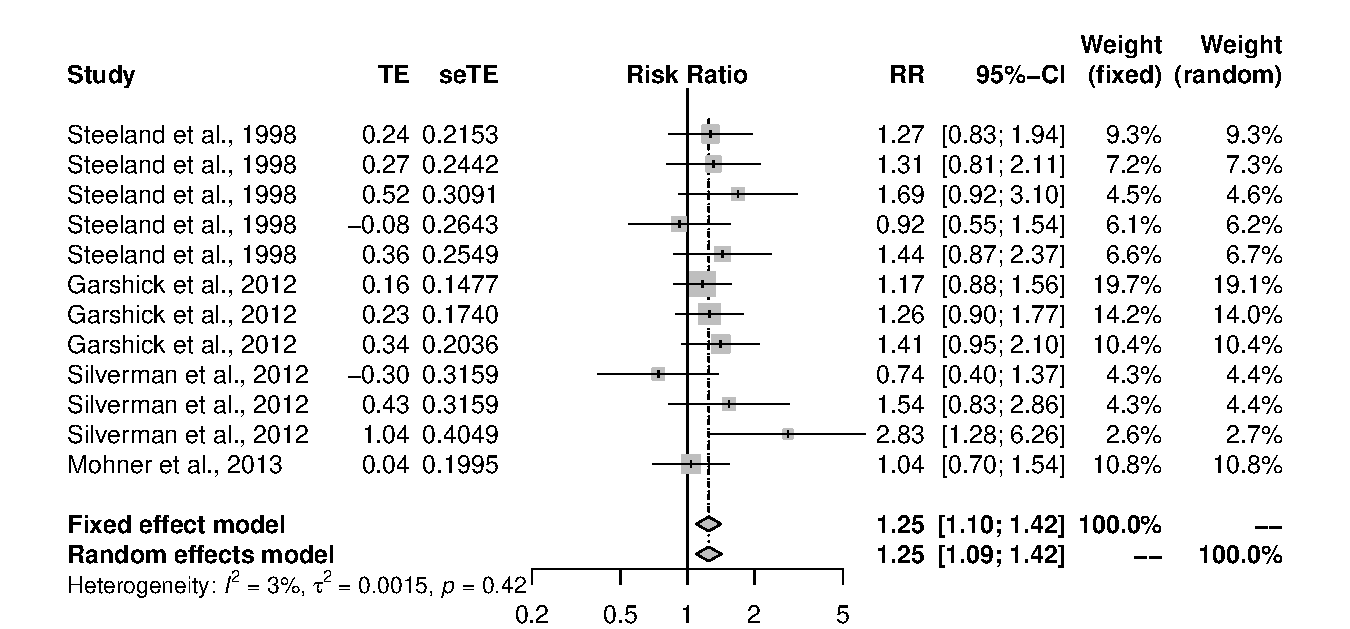
\includegraphics[width=.95\columnwidth]{fig3}
      \end{figure}
      \end{block}   
    \end{column}%2

    \begin{column}{0.36\linewidth}
      %-- Block 3-1
      \begin{block}{Environmental Fine PM-associated occupational mortality}
      To understand the ambient fine PM-associated the health risk of mortality, this study finds that the cardiovascular disease mortality and heart disease mortality are related to fine PM exposure for workers who have no occupational exposure to fine PM in the workplaces. However, we can only find few reference that focuses on the relationship between fine PM and occupational population.
      \vspace{5mm}
      \\
      {\large A) All-Cause Mortality}\\
      \begin{figure}[htb]
      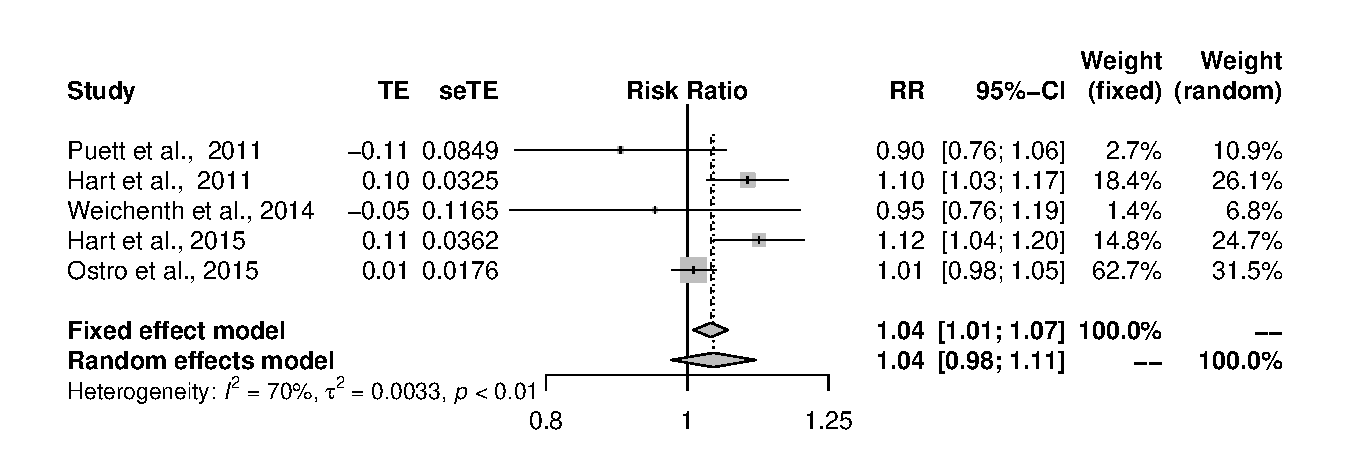
\includegraphics[width=.95\columnwidth]{fig5}
      \end{figure}
      {\large B) Cardiovascular Mortality}\\
      \begin{figure}[htb]
      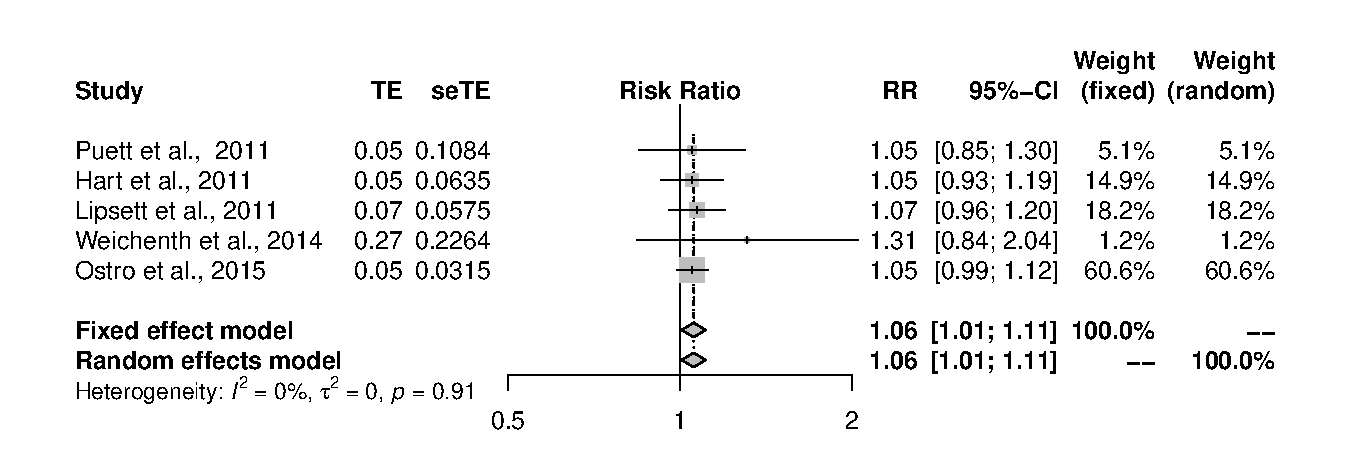
\includegraphics[width=.95\columnwidth]{fig6}
      \end{figure}
      {\large C) Heart Disease Mortality}\\
      \begin{figure}[htb]
      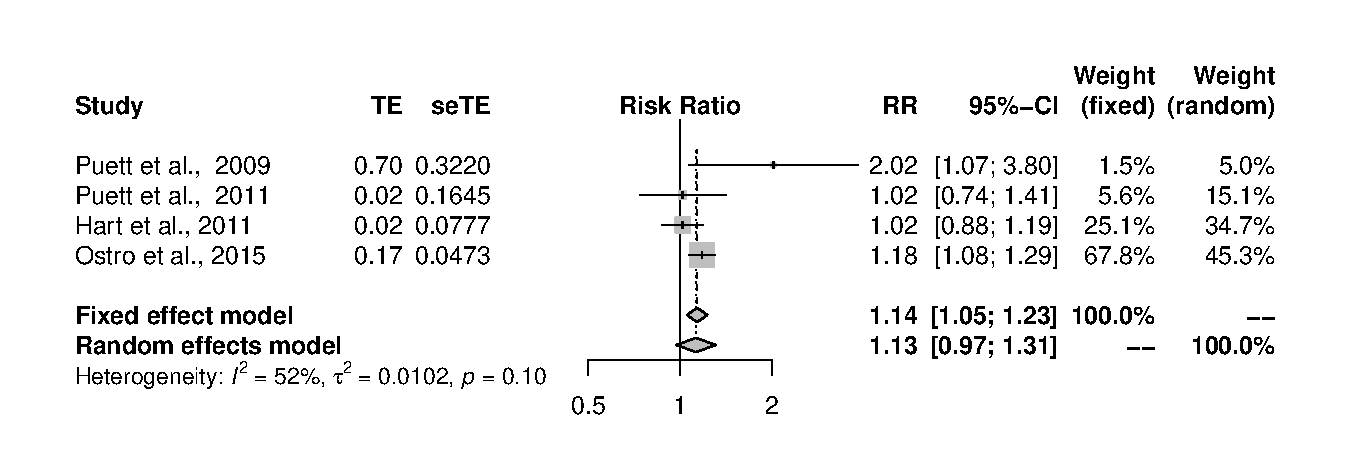
\includegraphics[width=.95\columnwidth]{fig7}
      \end{figure}
      \end{block}
      
      
%-- Block 3-3
      \begin{block}{Discussion}
        \begin{itemize}
          \item In this analysis, we focused attention on fine PM, which is prominent component of the air pollution. We divided the two different scenarios to quantify and understand the exposure risk for the occupational population. Current result shows that most studies had investigated the exposure risk of fine PM in the workplace. However, we also need to pay more attention to the occupational population who may have potential exposure risk to fine PM from ambient environment. 
          \item Most of the data were obtained from cohort studies; We did not place any restrictions based on whether or not a study adjusted for specific confounders. Therefore, homogeneity tests found the difference in estimates between exposure assessment techniques.
          \item A large number of hypothetical studies would be required to construct a symmetrical analysis and change the results of our meta-analyses.Results for mortality risk of lung cancer from fine PM was robust to influence analyses in occupational exposure, where the meta-estimate was recalculated with the systematic exclusion of each study.
        \end{itemize}
		\end{block}

      \begin{block}{Acknowledgements}
      The authors appreciate the useful discussion and suggestion from the members of Institute of Labor, Occupational Safety And Health, Ministry of Labor.
		\end{block}

%-- Block 3-4

      \begin{block}{Source code}
The R source code of this study were put on the github \url{https://github.com/nanhung/MetaPM}. We appreciate your valuable comments to improve this study.
		\end{block}

    \end{column}%3
  \end{columns}

\end{frame}
\end{document}


